
To better understand how coordination facts are used, we next present some programs that
take advantage of them. In our experimental setup, we used a machine with
four AMD Six-Core Opteron TM 8425 HE (2100 MHz) chips (24 cores) and 64 GB of
DDR-2 667MHz (16x4GB) RAM, running GNU/Linux (kernel 3.15.10-201 64 bits).
We compiled our virtual machine using GCC 4.8.3 (g++) with the flags
\texttt{-O3 -std=c++11 -fno-rtti -march=x86-64}~\footnote{Implementation
   available in \url{http://github.com/.../meld}}.

\subsection{Single Source Shortest Path}
Here we add coordination to the SSSP program described in \sectref{sect:ssspex}.
The coordinated version of the
SSSP~(Fig.~\ref{code:shortest_path_program_coord}) uses the coordination fact
\texttt{set-priority} (line 14). We also use a global program directive to order
priorities in ascending order (line 5).

When run with one thread, the algorithm behaves like
Dijkstra's shortest path algorithm~\cite{Dijkstra}. When using multiple
threads, each thread will pick the smallest distance from their subset of nodes.
While this does not yield the optimal program with relation to 1 thread, it
allows for parallel execution and locally avoids unnecessary work. The result
scales well and it is close to Dijkstra's algorithm.

\begin{topfig}
\scriptsize\begin{Verbatim}[numbers=left,commandchars=\\\{\}]
type route edge(node, node, int).
type linear shortest(node, int, list int).
type linear relax(node, int, list int).

\underline{priority @order asc}.

shortest(A, +00, []).
relax(@1, 0, [@1]).

shortest(A, D1, P1), D1 > D2, relax(A, D2, P2)
   -o shortest(A, D2, P2),
      \{B, W | !edge(A, B, W) |
         relax(B, D2 + W, P2 ++ [B]),
         \underline{set-priority(B, float(D2 + W))}\}.

shortest(A, D1, P1), D1 <= D2, relax(A, D2, P2)
   -o shortest(A, D1, P1).
\end{Verbatim}
  \scap{code:shortest_path_program_coord}{Shortest Path Program.}
\end{topfig}
\normalsize

The most interesting property of the SSSP program presented in
Fig.~\ref{code:shortest_path_program_coord} is that it remains provably correct,
although it applies rules using smarter ordering. The derivation of
\texttt{set-priority} does not change the behavior of the logical rules and the
code remains declarative.

Fig.~\ref{results:sssp_uspowergrid} shows experimental results when the
program computes the SSSP for 20\% of the nodes of the graph.
There are some situations where unnecessary facts are propagated
because although the shortest distance is selected locally, sub-optimal distances may be
propagated because many SSSP distances are computed at the same time.
However, we see a reduction of over 50\% in the number of
derived facts when using the coordinated version \textbf{C} over the regular
version \textbf{R}. The results also show that the coordinated
version using 16 threads is 1.3 times faster than the regular version using 16
threads while still showing good scaling.

\begin{topfig}
\vspace*{-5ex}
   \begin{center}
      \subfloat[]{ \begin{tabular}[b]{ | c | c | c | }
         \hline                       
         \textbf{\# T} & \textbf{R} & \textbf{C} \\ \hline \hline
         1 & 333K & 206K \\
         2 & 300K & 210K \\
         4 & 316K & 208K \\
         8 & 328K & 211K \\
         16 & 343K & 212K \\
         \hline  
         \end{tabular}
         \normalsize
      }
      \subfloat[]{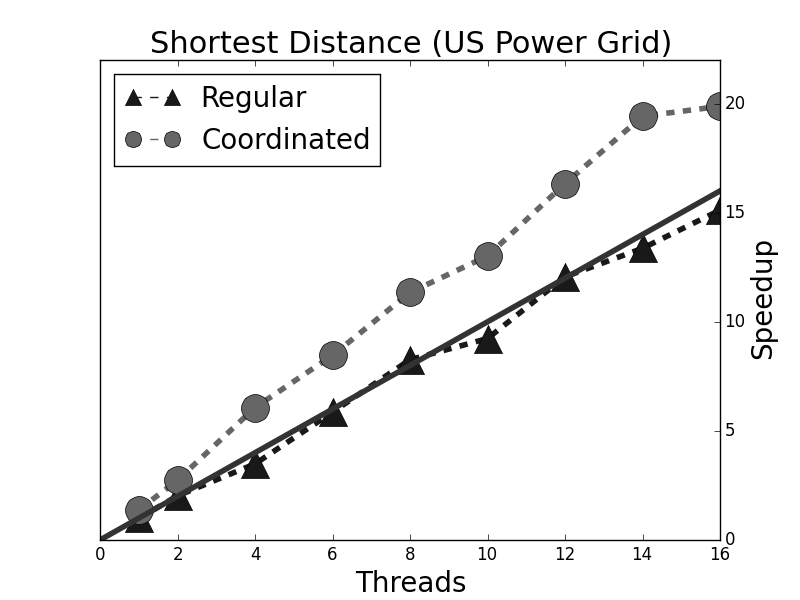
\includegraphics[width=5cm]{results/shortest-uspowergrid.png}}
   \end{center}
   \scap{results:sssp_uspowergrid}{Results for SSSP run on the 
   US power grid network.  On the left we show the number of facts
   derived for the regular \textbf{R} and coordinated
   version \textbf{C} using a variable number of threads \textbf{\#
   T}. On the right, we show the scalability of the regular and
   coordinated version. The speedup values are computed using the
   execution time for 1 thread.}
\vspace*{-3ex plus 0pt minus 1ex}
\end{topfig}


\subsection{MiniMax}
The MiniMax algorithm is a decision rule algorithm for minimizing the
possible loss for a worst case (maximum loss) scenario in a zero sum
game for 2 (or more) players that play in
turns~\cite{Edwards54}.

The algorithm builds a game tree, where each tree node represents a
game state and the children represent the possible game moves that can
be made by either player 1 or player 2.  An evaluation function is
used to compute the score of the board for each leaf of the tree. A
node is a leaf when the game state can no longer be expanded. Finally,
the algorithm recursively minimizes or maximizes the scores of each
node.  To select the best move for player 1, the algorithm picks the
move maximized at the root node.

In CLM, the program starts with a root node (with the initial game state)
that is expanded with the available moves at each level. The graph of the
program is dynamic since nodes are created and then deleted once they are no
longer needed. The latter happens when the
leaf scores are computed or when a node fully minimizes or maximizes the
children scores. When the program ends, only the root node has facts in its
database.

The code in Fig.~\ref{minimax:check-end} deals with the tree expansion process.
The first three rules (lines 1-10) deal
with the case where no children nodes are created and the last three rules
(12-29) deal with the cases that create new nodes. In particular, the two
rules in lines 12-26 generate new nodes using the
\mytt{exists} language construct, which creates a child node 
\mytt{B}. We link \mytt{B} with its parent (\mytt{parent(B, A)})
and kick start the expansion of that node \mytt{B} by adding a \mytt{play}
fact.

As noted in \sectref{sec:fifo}, the default scheduler is
breadth-first, which in this case leads to a complete expansion of the
tree before computing the scores at the leaves.  This results in using
$\mathcal{O}(n)$ memory, where $n$ is the number of nodes in the tree.

\begin{topfig}
\scriptsize\begin{Verbatim}[numbers=left,commandchars=\\\{\}]
expand(A, Board, [], 0, P, \underline{Depth})
  -o leaf(A, Board).

expand(A, Board, [], N, P, \underline{Depth}),
N > 0, P = player1
  -o maximize(A, N, -00, 0).

expand(A, Board, [], N, P, \underline{Depth}),
N > 0, P = player2
  -o minimize(A, N, +00, 0).

expand(A, Board, [0 | Xs], N, P, \underline{Depth}),
Depth >= 5
  -o exists B. (\underline{set-static(B)},
       \underline{set-default-priority(B, float(Depth + 1))},
       play(B, Board ++ [P | Xs], next(P), \underline{Depth + 1}),
       expand(A, Board ++ [0], Xs, N + 1, P, \underline{Depth}),
       parent(B, A)).

expand(A, Board, [0 | Xs], N, P, \underline{Depth}),
Depth < 5
  -o exists B. (
       \underline{set-default-priority(B, float(Depth + 1))},
       play(B, Board ++ [P | Xs], next(P), \underline{Depth + 1}),
       expand(A, Board ++ [0], Xs, N + 1, P, \underline{Depth}),
       parent(B, A)).

expand(A, Board, [C | Xs], N, P, \underline{Depth}) C <> 0
  -o expand(A, Board ++ [C], Xs, N, P, \underline{Depth}).
\end{Verbatim}
\scap{minimax:check-end}{MiniMax: checking if the game has ended and expanding the tree}
\vspace*{-2ex}
\end{topfig}
\normalsize

With coordination, we set the priority of a node to be its depth (lines 15 and
23) so that the tree is expanded in a depth-first fashion,
leading to a memory complexity of $\mathcal{O}(d t)$, where $d$
is the depth of the tree and $t$ is the number of threads.
Since threads prioritize deeper nodes, the scores of the first leaves are immediately
computed and then sent to the parent node. At this point, the leaves are deleted
and reused for other nodes in the tree, resulting in minimal memory usage.

\iffalse
As an example,
consider a system with 2 threads, $T_1$ and $T_2$, where $T_1$ first expands the root
node and then the first child. Since $T_2$ is idle, it steals half of the root's
children nodes and starts expanding one of the nodes in a depth-first fashion.
\fi

\iffalse
\begin{topfig}
   \begin{center}
      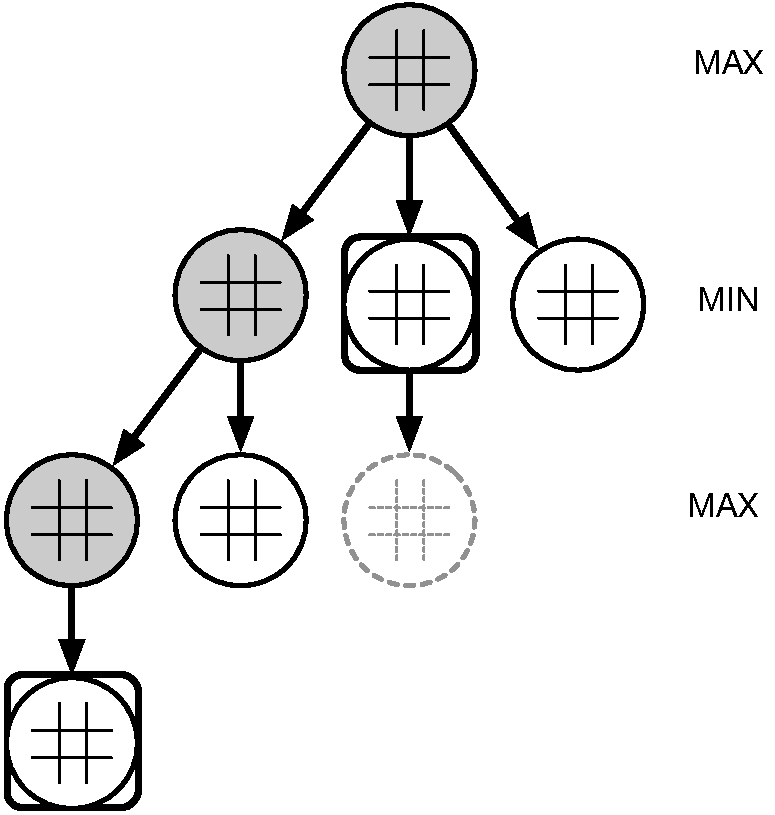
\includegraphics[width=4.5cm]{figures/minimax_tree}
   \end{center}
   \scap{fig:minimax}{Expanding the MiniMax tree using coordination. By prioritizing
      deeper nodes, threads are forced to expand the tree using a depth-first
      approach, which is superior since there is no need to expand the whole
      tree before computing the node scores.}
\end{topfig}
\fi

We also take advantage of memory locality by using \mytt{set-static} (line
14), so that nodes after a certain level are not stolen by other threads. While
this is not critical for performance in shared memory systems where node
stealing is fairly efficient, we expect that such coordination to be critical in
distributed systems.

\begin{topfig}
\vspace*{-3ex}
   \begin{center}
      \subfloat[]{\footnotesize\begin{tabular}[b]{ | c | c | c |}
         \hline                       
         \textbf{\# T} & \textbf{R} & \textbf{C} \\ \hline \hline
         1 & 11.80GB & 0.50MB \\ \hline
         2 & 12.19GB & 1.45MB \\ \hline
         4 & 13.82GB & 2.35MB \\ \hline
         8 & 14.87GB & 4.36MB \\ \hline
         16 & 13.79GB & 8.1MB \\ \hline
         \end{tabular}
         \normalsize
      }
      \subfloat[]{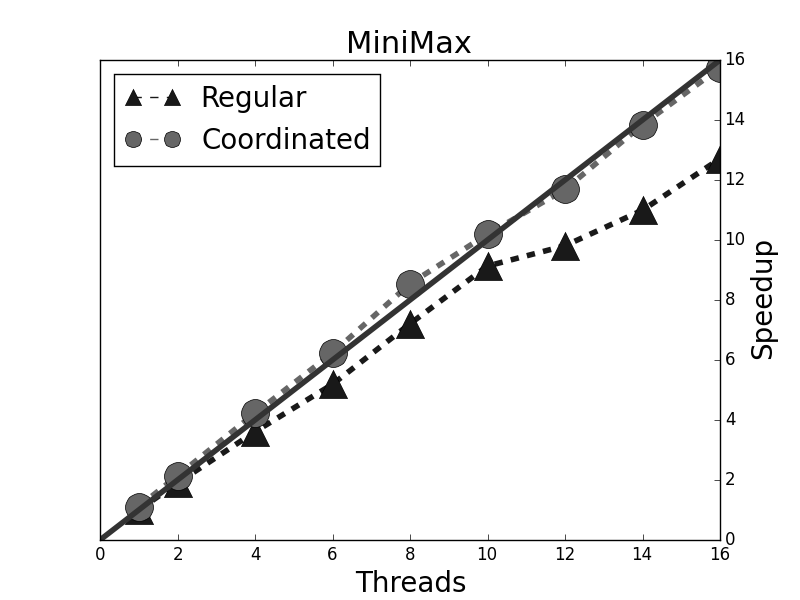
\includegraphics[width=4.5cm]{results/min-max-tictactoe.png}}
   \end{center}
   \scap{results:memory_minmax}{Memory usage and scalability of the regular and coordinated versions
      of MiniMax.}
\vspace*{-2ex}
\end{topfig}

In Fig.~\ref{results:memory_minmax} we compare the memory usage and scalability
of the coordinated MiniMax against the regular MiniMax. The coordinated version
uses significantly less memory (at most 8MB for 16 threads) than the regular
version (almost 14GB). Note that as the number of threads goes
up, memory usage also goes up. This is an artifact of our parallel memory
allocator that allocates large chunks of memory beforehand.
In terms of scalability, our experimental results show a 14-fold speedup for the
coordinated version against a 12-fold for the regular version when using 16
threads. When comparing the two versions directly, there is a 20\% run time
reduction when using 16 threads in the coordinated version.


\subsection{Heat Transfer}
In the Heat Transfer algorithm~(HT), we have a graph where heat values are
exchanged between nodes. The goal of the program is to exchange heat between
nodes. The program stops when the new heat values of every node are
$\delta = |H_i - H_{i-1}| \le \epsilon$. The algorithm works
asynchronously since heat values can be updated by using new partial information
coming from neighbor nodes. This increases parallelism since nodes do not need
to synchronize between iterations.

Fig.~\ref{code:ht} shows the HT rules that send new heat values to
neighbor nodes. In the first rule we added \texttt{add-priority} to increase the priority of the neighbor
nodes if the current node has a large $\delta$. The idea is to prioritize the
computation of heat values of nodes (using \texttt{update}) that have a neighbor
that changed significantly. Multiple \texttt{add-priority} facts will
increase the priority of a node so that nodes with multiple large deltas will
have more priority.

\begin{figure}[h!]
\scriptsize\begin{Verbatim}[numbers=left,commandchars=\\\[\]]
new-heat(A, New, Old),
Delta = fabs(New - Old),
Delta > epsilon
   -o {B, W | !edge(A, B, W) |
         new-neighbor-heat(B, A, New),
         update(B), \underline[add-priority(B, Delta)]}.

new-heat(A, New, Old)
fabs(New - Old) <= epsilon
   -o {B, W | !edge(A, B, W) |
         new-neighbor-heat(B, A, New)}.
\end{Verbatim}
  \caption{Coordination code for the Heat Transfer program. We updated the first rule
     to increase the priority of neighbor nodes.  The code logic remains exactly
     the same as before, however bigger changes in heat values are now
     propagated faster.}
  \label{code:ht}
\end{figure}
\normalsize

Fig.~\ref{results:ht} presents the scalability results for the uncoordinated
and coordinated version. The dataset used is a square grid with an inner square
with high heat nodes. With 1 thread, there's a 33\% reduction in run time, while
for 16 threads, there's a 18\% reduction.

To further improve locality, we split the second rule to
not send small $\delta$ values if the target node is in another
thread. XXX talk about results

\begin{figure}[h!]
\scriptsize\begin{Verbatim}[numbers=left,commandchars=\\\[\]]
new-heat(A, New, Old)
fabs(New - Old) <= epsilon
\underline[cpu-id(A, B, C)],
\underline[cpu-id(A, A, C)]
   -o {B, W | !edge(A, B, W) |
         new-neighbor-heat(B, A, New)}.

new-heat(A, New, Old)
fabs(New - Old) <= epsilon,
\underline[cpu-id(A, B, C1)],
\underline[cpu-id(A, A, C2)],
\underline[C1 <> C2]
   -o 1. // nothing is derived
\end{Verbatim}
  \caption{To improve locality, we added a third rule to not send small $\delta$
     values if the neighbor is in another thread.}
  \label{code:ht_better}
\end{figure}
\normalsize

\begin{figure}[ht!]
   \begin{center}
      \subfloat[]{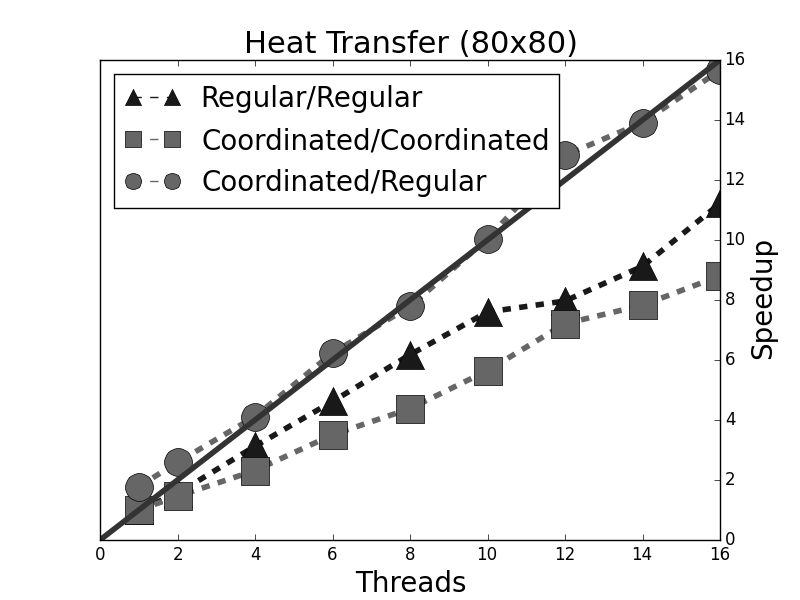
\includegraphics[width=5cm]{results/new-heat-transfer-80}}
   \end{center}
   \caption{Experimental results for the HT program. The coordinated version
      is, on average, 30\% faster than the regular version although it has a
      slightly worse scalability due to a reduction in work available.}
   \label{results:ht}
\end{figure}


\subsection{Splash Belief Propagation}
Randomized and approximation algorithms can obtain significant benefits from
coordination directives because their inherent non-determinism can be harnessed
to evaluate rules in different orders.
An example of such program is Loopy Belief Propagation.
Loopy Belief Propagation~\cite{Murphy99loopybelief} (LBP) is an approximate inference algorithm
used in graphical models with cycles. In its essence, LBP is a sum-product message passing algorithm
where nodes exchange messages with their immediate neighbors and apply some computations to the messages
received.

LBP is an algorithm that maps very well to the graph based model of CLM. In its
original form, the belief values of nodes are computed by synchronous iterations.
LBP offers more concurrency when belief values are computed asynchronously
leading to faster convergence. For this, every node keeps track of all messages
sent/received and recomputes the belief using partial information from neighbor
nodes. It is then possible to prioritize the computation of beliefs when a
neighbor's belief changes significantly.

The asynchronous approach proves to be a nice improvement over the synchronous
version. Still, it is possible to do even better. Gonzalez et
al~\cite{Gonzalez+al:aistats09paraml} developed an optimal algorithm to compute
this algorithm by first building a tree and then updating the beliefs of each
node twice, first from the leaves to the root and then from the root to the
leaves. The root of this tree is the node with the highest priority (based on
belief) while the other nodes in the tree must have a non-zero priority.
Note that the priorities are updated whenever a neighbor updates their belief.
These \emph{splash trees} are built iteratively until we reach convergence.
%In Fig.~\ref{splash_bp} we represent two threads creating two different splash trees.

\iffalse
\begin{topfig}
   \begin{center}
      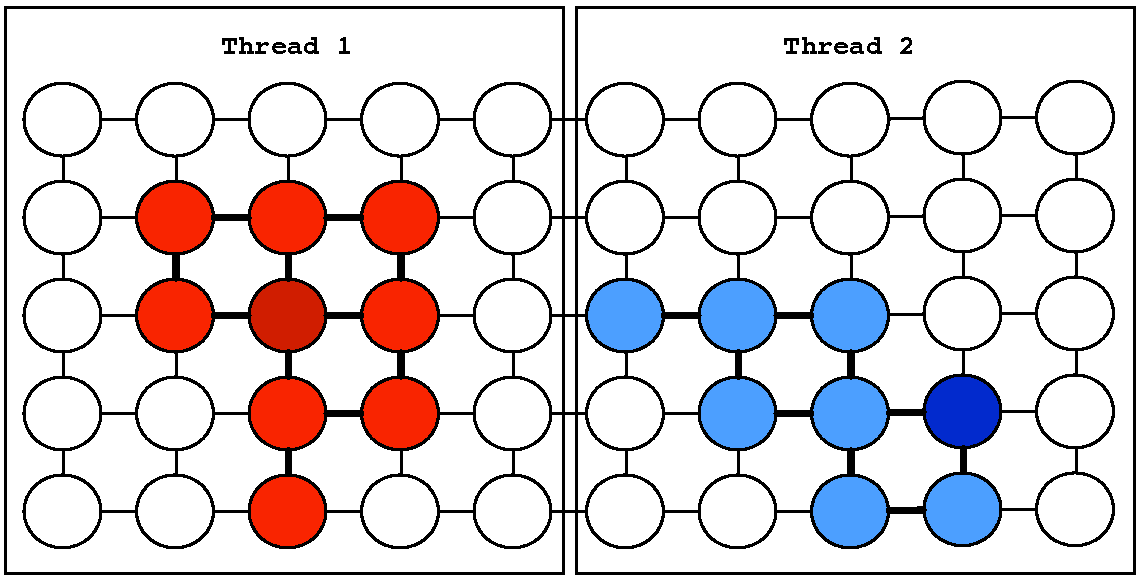
\includegraphics[width=6.5cm]{figures/splash_bp}
   \end{center}
   \scap{splash_bp}{Creating splash trees for belief propagation. Each threads picks the
   highest priority node and creates a tree from that node. The belief values
   are updated in two phases: first from the leaves to the root and then from
   the root to the leaves.}
\end{topfig}
\fi

The code for Splash Belief Propagation~(SBP) in Fig.~\ref{code:sbp} presents the
coordination code for LBP.  Please note that we just appended the code in
Fig.~\ref{code:sbp} to a working but unoptimized version of the algorithm, every
other rule remains the same. We add new rules that coordinate
the creation and execution of the splash trees:

\begin{tightdescription}
   \item[Tree building]: Each node has a \texttt{inactive} fact that is used to
   start the tree building process. When the highest priority node is picked, a
   \texttt{tree} is created that will navigate through the tree. In lines 15-21,
   we use an \emph{aggregate}~\cite{cruz-iclp14} to gather all the neighbor
   nodes that have a positive priority (due to a new belief update) and are in the
   same thread. Nodes are collected into list \texttt{L} (line 21) and
   appended to list \texttt{Next}.
   
   \item[First phase]: In the
   third rule (lines 11-12), when the number of nodes of the tree reaches a
   certain limit, a \texttt{first-phase} is generated to update the beliefs of
   all nodes in the tree, starting from the leaves and ending at the root As the
   nodes are updated, an \texttt{update} fact is derived to update the belief
   values (line 35).

   \item[Second phase]: In the second phase, the computation of beliefs is
   performed from the root to the leaves and the belief values are updated a
   second time (line 42).
\end{tightdescription}

The \texttt{set-static} and \texttt{set-cpu} action facts are used in
line 2 to (1) force nodes to stay in the thread and (2) 
partition nodes as a grid of threads. This sets up well defined areas
of nodes for threads to build splash trees on.

\begin{topfig}
\scriptsize\begin{Verbatim}[numbers=left,commandchars=*\{\}]
!coord(A, X, Y), start(A)
   -o *underline{set-static(A), set-cpu(A, grid(X, Y))}.

// TREE BUILDING
// expand tree by adding neighbor nodes
inactive(A), tree(A, All, Next) -o expand-tree(A, All, Next).
// start tree since we do not have one
inactive(A), *underline{@priority(A, A, P)}, P > 0.0
   -o expand-tree(A, [A], [A]).
// end tree building
expand-tree(A, All, Next), length(All) >= maxnodes
   -o first-phase(A, All, reverse(All)).
// expand tree
expand-tree(A, All, [A | Next]), length([A | Next]) < maxnodes
   -o [collect => L | Side | !edge(A, L, Side),
         0 = count(All, L), // L is not in All
         0 = count(Next, L), // L is not in Next
         *underline{@priority(A, L, P), P > 0.0,}
         *underline{@cpu-id(A, L, Id1)},
         *underline{@cpu-id(A, A, Id2), Id1 = Id2} |
         send-tree(A, All, Next ++ L)].

send-tree(A, All, [])
   -o first-phase(A, All, reverse(All)).
send-tree(A, All, [B | Next])
   -o *underline{schedule-next(B)},
      tree(B, All ++ [B], [B | Next]).

// FIRST PHASE
first-phase(A, [A], [A]) -o second-phase(A, [], A).
first-phase(A, [A, B | Next], [A])
   -o update(A), *underline{schedule-next(B)},
      second-phase(B, [B | Next], A).
first-phase(A, All, [A, B | Next])
   -o update(A), *underline{schedule-next(B)},
      first-phase(B, All, [B | Next]).

// SECOND PHASE
second-phase(A, [], _)
   -o *underline{set-priority(A, 0.0)}, inactive(A), update(A).
second-phase(A, [A], Back)
   -o update(A), inactive(Back),
      inactive(A), *underline{set-priority(A, 0.0)}.
second-phase(A, [A, B | Next], Back)
   -o update(A), inactive(Back), *underline{schedule-next(B)},
      second-phase(B, [B | Next], A).
\end{Verbatim}
  \scap{code:sbp}{Coordination code for the Splash Belief Propagation program. 
%CLM needs 50 lines of rules to implement splash trees, while GraphLab needs a total of 350 lines of C++ to implement the same functionality.
  Note
     that when a linear fact is prefixed by \texttt{@}, it indicates that the
     fact is going to be re-derived.}
\end{topfig}
\normalsize

\begin{dblfig}
   \begin{center}
      \subfloat[]{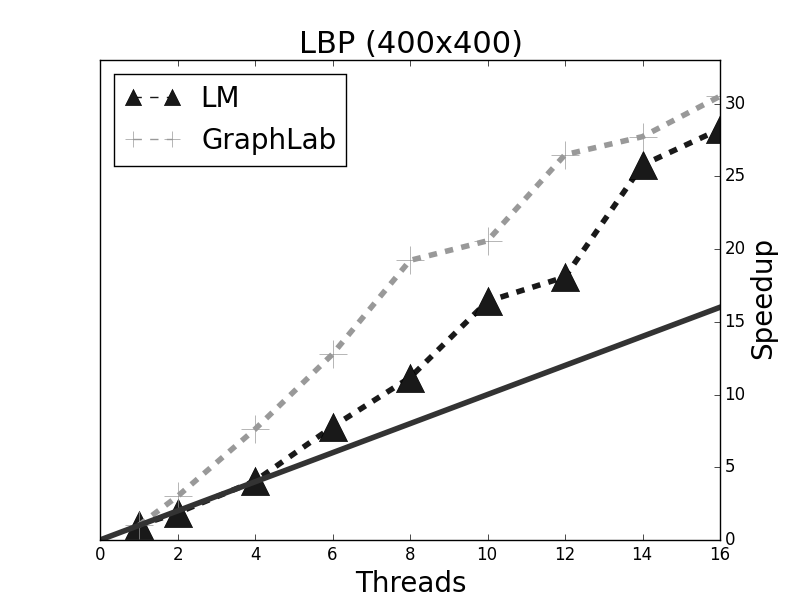
\includegraphics[width=5.5cm]{results/system_belief-propagation-400.png}}
      \subfloat[]{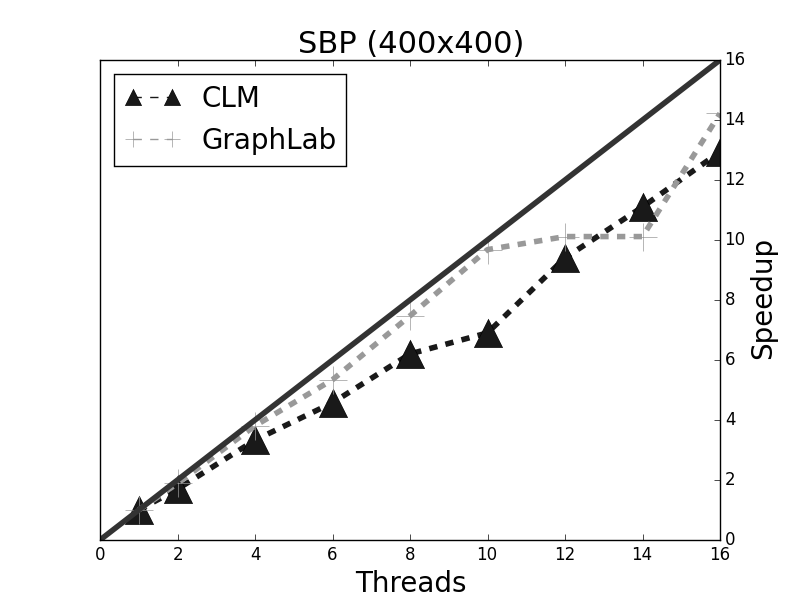
\includegraphics[width=5.5cm]{results/system_splash-bp-400.png}}
      \subfloat[]{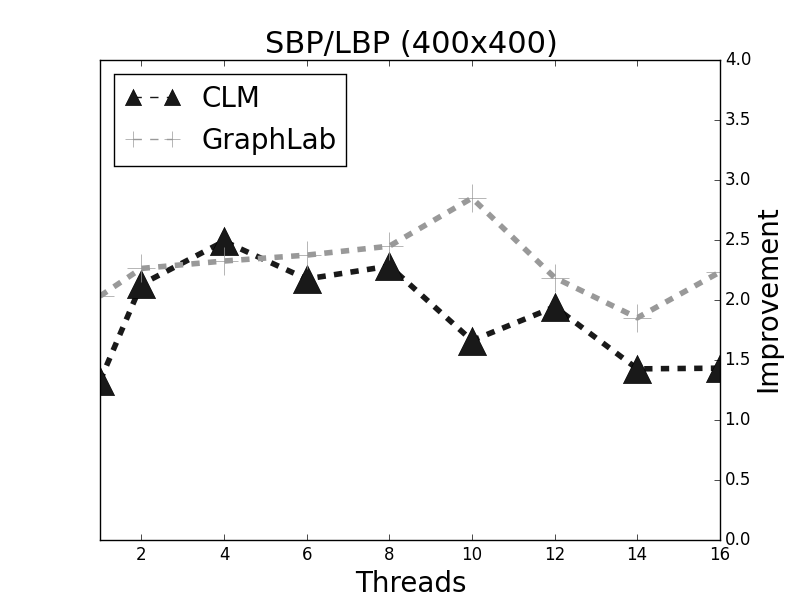
\includegraphics[width=5.5cm]{results/system_improve_belief-propagation-400.png}}
   \end{center}
   \scap{results:splash_bp}{Experimental results for LBP and SBP. (a) shows the
      scalability of LBP for both CLM and GraphLab and (b) shows the
      scalability of SBP. (c) presents the
      improvements seen in SBP against LBP, where SBP runs, on average, 1.5 to 2.5
      times faster than LBP.}
\end{dblfig}

In this program, coordination assumes a far more important role than
we have seen before. Coordination rules fully drive the behavior of
the algorithm and although the final result of the algorithm is
statistically identical to the original algorithm, SBP works very
differently than LBP.  SBP is also implemented in
GraphLab~\cite{GraphLab2010}, a C++ framework for writing machine
algorithms.  GraphLab provides the splash scheduler as part its the
framework. It is 350 lines of C++ code.  With our coordination facts,
it is possible to create the necessary scheduling with only 12 rules.

We measured the behavior of LBP and SBP for both CLM and GraphLab.
Fig.~\ref{results:splash_bp} shows that both systems have very similar behavior
when using a variable number of threads.  The differences in performance between
GraphLab and CLM comes mainly because GraphLab performs in-place updates of
neighbor belief values, while CLM compiler and runtime system performs naive
manipulation of facts by deriving rules. The in-place update could be generated
by the compiler using smarter compilation strategies.


\subsection{N Queens}
The N-Queens puzzle is the problem of placing N chess queens on an NxN
chessboard so that no pair of two queens attack each
other~\cite{8queens}. The challenge of finding all the
distinct solutions to this problem is a well-known benchmark in designing
parallel algorithms.

The CLM solution considers the squares of the chess board as a graph
of nodes which exchange valid configurations with each
other. Initially every square in the first row of the board gets the
empty state.  Then, each square adds its own position to the state and
sends the state down, to the next row. Once a square receives new
configurations, it attempts to add its position to the
configurations. If valid, that configuration is then sent,
recursively, to the next row, until all rows are traversed. At the end
of the program, the squares at the bottom row will have all the valid
configurations.

Since computation goes from the top row to the bottom row, not all placements of
nodes to threads perform equally. This is especially true because the bottom
rows tend to perform the most work. The best placement is then to split the
board vertically with axiom \mytt{set-cpu(A, vertical(X, Y))} so each thread
gets the same number of columns, where \mytt{X} and \mytt{Y} are the coordinates
of the board. Our experiments show that, on a shared memory system, it does not
matter much if we start with a bad placement since node stealing overcomes those
issues by load balancing dynamically.  However, the N Queens program
incrementally builds and shares lists representing valid board states that are
transmitted from top to bottom.  In order to improve memory locality we should
then manipulate board states that share a significant number of elements because
each board state needs to be iterated before extended with a new position.  To
accomplish this, we used coordination axioms \mytt{set-default-priority(A, X)},
where \mytt{X} is the row number (0 is the top row) in order to
prioritize the evaluation of squares closer to the bottom of the
board.

Experimental results are presented in Fig.~\ref{results:nqueens}.  We
first ran the coordinated program using dynamic partitioning (with
work stealing) and saw some performance improvements
(\textbf{Coordinated}). However, using dynamic partitioning is bad for
memory locality since threads will often steal nodes.  We then
added \mytt{set-static(A)} as a coordination axiom (line
\textbf{Static/Regular}) and saw a significant drop in data cache misses and an
improvement in performance, specially when using 13 threads (the number of
columns).

\begin{topfig}
\vspace*{-1ex}
   \begin{center}
      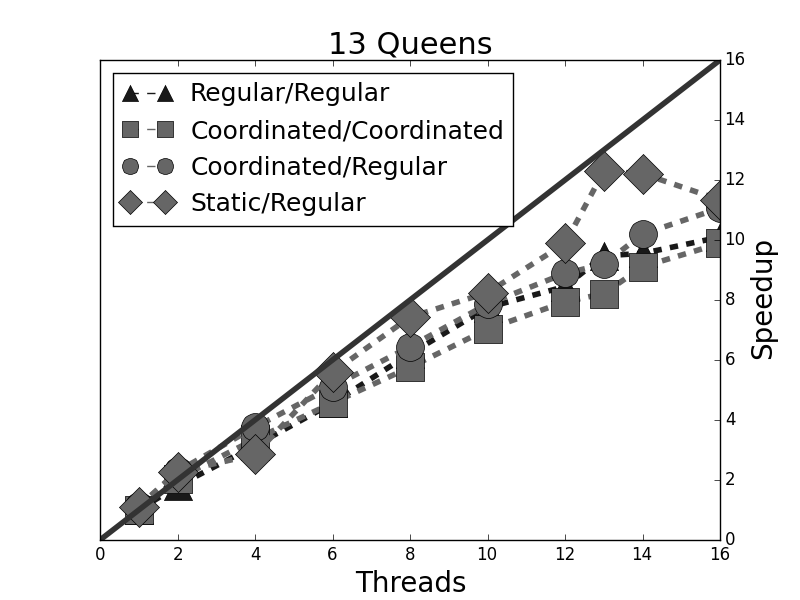
\includegraphics[width=\figsize]{results/8queens-13.png}
   \end{center}
   \scap{results:nqueens}{Experimental results for the 13 Queens program.
   Coordination works best when 1 column is assigned to one thread and bottom
   rows have higher priority.}
\end{topfig}

